\section{Recursos e M�todos}

\definecolor{LightCyan}{rgb}{0.88,1,1}


%A metodologia � a aplica��o de procedimentos e t�cnicas que devem ser observadas
para constru��o do conhecimento de comprovar sua validade e utilidade nos
diversos �mbitos da sociedade. Em em um n�vel aplicado, examina, descreve e
avalia m�todos e t�cnicas de pesquisa que possibilitam a coleta e o
processamento de informa��es, visando ao encaminhamento e � resolu��o de temas
de investiga��o \cite{MetodologiaCientifica}.
Pesquisa cient�fica � a realiza��o de um estudo planejado, sendo o m�todo de
abordagem do problema, o que caracteriza o aspecto cient�fico da investiga��o.
Sua finalidade � descobrir respostas para quest�es mediante a aplica��o do
m�todo cient�fico. A pesquisa sempre parte de um problema, uma interroga��o ou
uma situa��o para a qual o repert�rio de conhecimento dispon�vel n�o gera
resposta adequada. Para solucionar esse problema, s�o levantadas hip�teses que
podem ser confirmadas ou refutadas pela pesquisa. Portanto, toda pesquisa se
baseia em uma teoria que sirva como ponto de partida para a investiga��o.
Utilizando-se de formas tradicionais de classifica��o das pesquisas, temos uma
compila��o como mostrado na Figura~\ref{fig:tiposdepesquisa}
\cite{MetodologiaCientifica}.


\begin{figure}[h!]
\centering
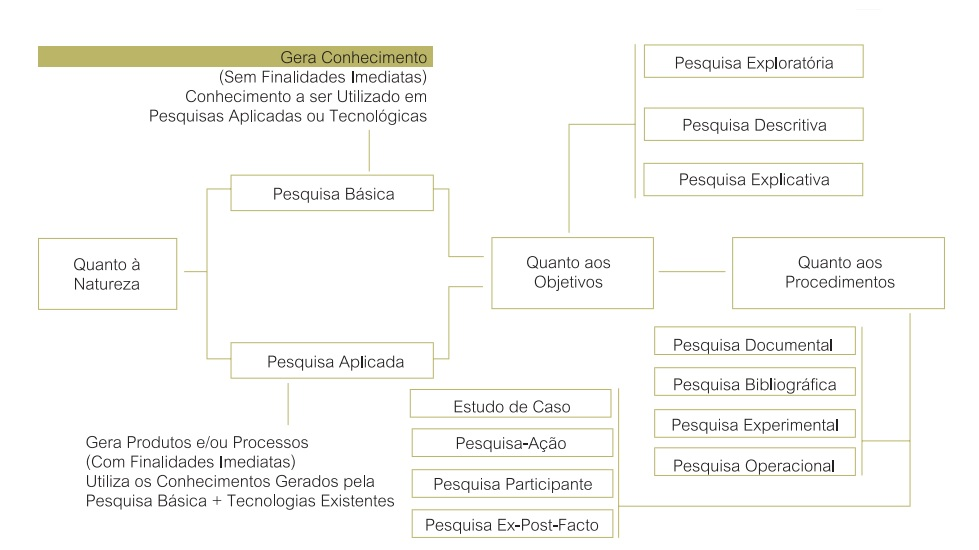
\includegraphics[scale=0.5]{images/tiposdepesquisa}
\caption{Categorias de pesquisas cient�ficas. Fonte
\cite{MetodologiaCientifica} }
\label{fig:tiposdepesquisa}
\end{figure}


A tabela~\ref{table:classificacaopesquisa} sumariza como o presente trabalho se
categoriza segundo o m�todo tradicional de classifica��o dos crit�rios


\definecolor{LightCyan}{rgb}{0.88,1,1}


 \begin{table}[H]
  \centering
      \caption{Classifica��o da pesquisa}
\label{table:classificacaopesquisa}
    \begin{tabular}{|l|l|}
    \hline
    \rowcolor{LightCyan}
     Ponto de Vista & Tipo de pesquisa utilizada   \\
     \hline
    Natureza   & Pesquisa Aplicada     \\
    Abordagem do Problema   & Pesquisa Quantitativa        \\
    Objetivos  & Pesquisa Explicativa \\
    Procedimentos T�cnicos  & Pesquisa Bibliogr�fica, Pesquisa
    Experimental 
    \\
    \hline
    \end{tabular}

\end{table}


\begin{enumerate}
  \item  \textbf{Natureza}\newline
  A pesquisa aplicada objetiva gerar conhecimentos para aplica��o pr�tica,
  dirigidos � solu��o de problemas espec�ficos \cite{MetodologiaCientifica}.
  Assim, a pesquisa sobre reconhecimentos de padr�o aplicados � realidade
  aeron�utica, tem como objetivo selecionar as t�cnicas mais adequadas para
  situa��es reais em futuras aplica��es de AR para manuten��o, portanto se
  categoriza como uma aplica��o pr�tica a um problema espec�fico.
  
  \item \textbf{Abordagem do Problema}\newline
  A pesquisa quantitativa, tem como objetivo garantir a precis�o dos
  resultados, evitando contradi��es no processo de an�lise e interpreta��o, para tanto � feita uma
  hip�tese pr�via e tra�ada uma estrat�gia para prov�-la.
    O estudo da melhor t�cnica de reconhecimento de padr�es � realizada com
  experimentos emp�ricos e seu ambiente � artificial, emulando situa��es que,
  caso feitos de forma natural, demandariam muito tempo e custo, pois deveriam
  ser realizados em diversas aeronaves e em diversos ambientes, desde cen�rios
  noturnos at� cen�rio com neve.  
  
  \item \textbf{Objetivos}\newline
  A pesquisa explicativa tem por objetivo explicar
  os porqu�s das coisas e suas causas, por meio do registro, da an�lise, da classifica��o e da
  interpreta��o dos fen�menos observados. Visa identificar os fatores que
  determinam ou contribuam para a ocorr�ncia dos fen�menos; ''aprofunda o
  conhecimento da realidade porque explica a raz�o, o porqu� das
  coisas.'' \cite{ElaborarPesquisa}.

    
  \item \textbf{Procedimentos T�cnicos}\newline
  Este trabalho utiliza as seguintes formas de procedimentos: Pesquisa
  Bibliogr�fica e Pesquisa Experimental.
  A pesquisa bibliogr�fica � elaborada a partir de material j� publicado,
  constitu�do principalmente de: livros, revistas, publica��es em peri�dicos e
  artigos cient�ficos, jornais, boletins, monografias, disserta��es,teses,
  material cartogr�fico e internet, sempre com o objetivo de proporcionar ao
  pesquisador um contato direto com todo material j� existente sobre o assunto
  da pesquisa. Para elaborar o presente trabalho, foi feita uma intensa
  busca por t�cnicas de reconhecimento de padr�o com o objetivo de posterior uso
  em aplica��es de AR e sobre o uso de AR na manuten��o e compara��es
  de t�cnicas em outros contextos que n�o o aeron�utico.
  Na Pesquisa Experimental determinamos um objeto de estudo, selecionamos as
  vari�veis que seriam capazes de influenci�-lo e definimos as formas de
  controle e de observa��o dos efeitos que a vari�vel produz no objeto. No presente trabalho, foram gerados
  experimentos refazendo situa��es reais, avaliando o impacto de vari�veis
  ambientais por meio de aproxima��es matem�ticas aos eventos reais, como por exemplo, varia��o de brilho,
   escala ou rota��o do ponto de vista do usu�rio em rela��o ao objeto de
   estudo.
  
  
\end{enumerate}


Com uma abordagem pragm�tica, temos a tabela~\ref{table:metodosresumo}, que
exemplifica para cada um dos objetivos os recursos utilizados e os m�todos com
os quais ser�o atingidos.

\begin{table}[H]
  \centering
      \caption{Resumo de Recursos e M�todos}
      \label{table:metodosresumo}
    \begin{tabular}{|m{150pt}|m{100pt}|m{150pt}|}
     \rowcolor{LightCyan}
    \hline
    Objetivo & Recurso & M�todo\\
     \hline
     Avaliar os algoritmos cl�ssicos de reconhecimento & Artigos, Livros e Sites
     & Pesquisa Bibliogr�fica
     \\
     \hline
    Aplicar os algoritmos cl�ssicos � situa��es reais   & Recursos fornecidos
    pelo OpenCV & Simula��es
    \\
    \hline
    Selecionar algoritmo mais adequado para o contexto & Dados coletados de
    simula��o & An�lise de cad�ncia e qualidade de reconhecimento\\
   \hline
     \end{tabular}
\end{table}




